\documentclass[11pt,a4paper]{article}

\usepackage[margin=2.4cm]{geometry}
\usepackage{amsmath,amssymb,amsthm,mathtools}
\usepackage{enumitem}
\usepackage{booktabs}
\usepackage{array}
\usepackage{tikz}
\usetikzlibrary{automata,positioning,arrows.meta,calc}
\usepackage{microtype}
\usepackage{setspace}
\usepackage[hidelinks]{hyperref}
\usepackage{fancyhdr}

\onehalfspacing
\setlength{\parskip}{0.35em}
\setlength{\parindent}{0pt}

\newtheorem{theorem}{Theorem}[section]
\newtheorem{lemma}[theorem]{Lemma}
\newtheorem{corollary}[theorem]{Corollary}
\newtheorem{proposition}[theorem]{Proposition}
\theoremstyle{definition}
\newtheorem{definition}[theorem]{Definition}
\newtheorem{example}[theorem]{Example}
\newtheorem{exercise}[theorem]{Exercise}
\newtheorem{algorithm}[theorem]{Algorithm}
\theoremstyle{remark}
\newtheorem{remark}[theorem]{Remark}

\newcommand{\emptystring}{\varepsilon}
\newcommand{\powerset}[1]{\mathcal{P}(#1)}
\newcommand{\lang}[1]{L(#1)}
\newcommand{\concat}{\mathbin{\cdot}}
\newcommand{\transition}{\delta}
\newcommand{\set}[1]{\{#1\}}
\newcommand{\cfl}{\mathrm{CFL}}
\newcommand{\eps}{\varepsilon}
\newcolumntype{L}[1]{>{\raggedright\arraybackslash}p{#1}}

\tikzset{
  automaton/.style={
    >={Stealth[scale=0.85]},
    thick,
    auto,
    initial text=,
    node distance=27mm,
    every state/.style={minimum size=8.8mm, inner sep=1pt, font=\small},
    every loop/.style={looseness=7, min distance=7mm},
    every edge/.style={draw,->,thick}
  },
  box/.style={
    draw,
    rounded corners,
    align=center,
    minimum height=11mm,
    minimum width=22mm,
    font=\small
  },
  arrow/.style={-{Stealth},thick}
}

\pagestyle{fancy}
\fancyhf{}
\setlength{\headheight}{14pt}
\lhead{MTL783}
\rhead{Theory of Computation}
\cfoot{\thepage}

\title{\textbf{MTL783}\\[0.4em]
Theory of Computation}
\author{}
\date{}

\begin{document}
\maketitle
\tableofcontents
\newpage

\section*{Course information}
\addcontentsline{toc}{section}{Course information}
\textbf{Course.} MTL783, Theory of Computation.

\textbf{Assessment.}
\begin{center}
\begin{tabular}{@{}lc@{}}
\toprule
Component & Weight\\
\midrule
Quiz & $20\%$\\
Minor & $35\%$\\
Major & $40\%$\\
Attendance & $5\%$\\
\bottomrule
\end{tabular}
\end{center}

\section{Foundations: alphabets, strings, and computation}

\subsection{What is computation?}
A computation is the process by which an abstract machine reads an input
string, updates a finite (or unbounded) internal configuration, and eventually
answers accept or reject. The course studies three models of
increasing memory:
\begin{enumerate}
  \item \textbf{Finite automata} --- finite memory, encoded entirely in the
        current state.
  \item \textbf{Pushdown automata} --- finite control plus a stack.
  \item \textbf{Turing machines} --- unbounded tape memory.
\end{enumerate}
Finite automata correspond to regular languages; pushdown automata to
context-free languages; Turing machines to the recursively enumerable languages.
The first two models occupy these notes; Turing machines come later in the
course.

\subsection{Alphabets, strings, and languages}
\begin{definition}[Alphabet and strings]
An \emph{alphabet} $\Sigma$ is a finite nonempty set of symbols. A
\emph{string} over $\Sigma$ is a finite sequence of symbols from $\Sigma$.
The empty string is $\eps$, and $|\eps|=0$. Write $|w|$ for the length of
$w$. Concatenation of $u$ and $v$ is written $uv$.
\end{definition}

The set of all strings over $\Sigma$ is $\Sigma^*$. Formally
\[
  \Sigma^0=\set{\eps},\qquad
  \Sigma^{n+1}=\set{wa:w\in\Sigma^n,\,a\in\Sigma},\qquad
  \Sigma^*=\bigcup_{n\geq 0}\Sigma^n.
\]
Write $\Sigma^+=\Sigma^*\setminus\set{\eps}$ for the nonempty strings.

\begin{definition}[Language]
A \emph{language} over $\Sigma$ is any subset $L\subseteq\Sigma^*$.
\end{definition}

Two equivalent viewpoints appear throughout the notes.
\begin{itemize}
  \item A machine $M$ that takes strings over $\Sigma$ as input defines
        \[
          \lang{M}=\set{w\in\Sigma^*:M\text{ accepts }w}.
        \]
  \item A function $f:\Sigma^*\to\set{0,1}$ defines
        \[
          L_f=\set{w\in\Sigma^*:f(w)=1}.
        \]
\end{itemize}
Recognition is the special case of computing a Boolean function on strings.

\subsection{First look at finite automata}
A finite automaton is drawn as a \emph{state diagram}:
\begin{itemize}
  \item circles are states;
  \item a double circle is an accept state;
  \item arrows are transitions, labelled by input symbols;
  \item an incoming arrow with no source marks the start state;
  \item the output of a completed run is accept/reject
        (equivalently yes/no).
\end{itemize}

\begin{example}[The machine $M_1$]
Let $\Sigma=\set{0,1}$ and let $M_1$ have states $\set{q_1,q_2,q_3}$, start
state $q_1$, and sole accept state $q_2$.
\begin{center}
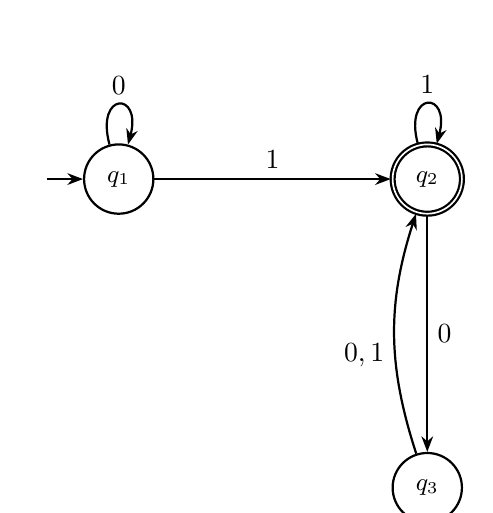
\begin{tikzpicture}[automaton,node distance=30mm]
  \node[state,initial] (q1) {$q_1$};
  \node[state,accepting,right=of q1] (q2) {$q_2$};
  \node[state,below=of q2] (q3) {$q_3$};
  \path[->]
    (q1) edge[loop above] node{$0$} ()
         edge node[above]{$1$} (q2)
    (q2) edge[loop above] node{$1$} ()
         edge node[right]{$0$} (q3)
    (q3) edge[bend left=18] node[below left]{$0,1$} (q2);
\end{tikzpicture}
\end{center}
$M_1$ accepts precisely those strings that contain at
least one $1$, after which an even number of $0$s occur. Equivalently: after
the last $1$, the number of trailing $0$s is even (including the case of no
trailing $0$s, i.e.\ strings that end in $1$).

Sample runs:
\[
\begin{array}{c|ccccc}
\text{input} & 1 & 01 & 11 & 010 & 0100\\
\hline
\text{end state} & q_2 & q_2 & q_2 & q_3 & q_2\\
\text{result} & \text{accept} & \text{accept} & \text{accept} & \text{reject} & \text{accept}
\end{array}
\]
The diagram determines a unique language: all $w$ such that
$\transition^*(q_1,w)=q_2$.
\end{example}

\section{Deterministic finite automata}

\subsection{Formal definition}
\begin{definition}[DFA]
A \emph{deterministic finite automaton} is a $5$-tuple
\[
  M=(Q,\Sigma,\transition,q_0,F)
\]
where
\begin{enumerate}
  \item $Q$ is a finite set of states;
  \item $\Sigma$ is a finite alphabet;
  \item $\transition:Q\times\Sigma\to Q$ is the \emph{transition function};
  \item $q_0\in Q$ is the start state;
  \item $F\subseteq Q$ is the set of accept states.
\end{enumerate}
\end{definition}

Two remarks:
\begin{enumerate}
  \item $F$ may be empty. Then $\lang{M}=\varnothing$: no string is accepted.
  \item Determinism means that for every pair $(q,a)\in Q\times\Sigma$ there is
        \emph{exactly one} next state $\transition(q,a)$.
\end{enumerate}

\begin{example}[The $5$-tuple for $M_1$]
\[
\begin{array}{rl}
  Q&=\set{q_1,q_2,q_3},\\
  \Sigma&=\set{0,1},\\
  q_0&=q_1,\\
  F&=\set{q_2},
\end{array}
\qquad
\begin{array}{c|cc}
\transition & 0 & 1\\
\hline
q_1 & q_1 & q_2\\
q_2 & q_3 & q_2\\
q_3 & q_2 & q_2
\end{array}
\]
If $M$ accepts a set $A$, we call $A$ the \emph{language of} $M$ and write
$A=\lang{M}$.
\end{example}

\subsection{A modulo-3 machine with RESET}
\begin{example}[Running sum modulo $3$]
Let $\Sigma=\set{0,1,2,\mathtt{RESET}}$. Think of $0,1,2$ as adding that
value to a running total, and of $\mathtt{RESET}$ as setting the total back
to $0$. Accept if the current total is $0\bmod 3$.

States $q_0,q_1,q_2$ store the current residue. The start and accept state is
$q_0$. Transitions on $1$ and $2$ move around the triangle; $0$ is a self-loop;
$\mathtt{RESET}$ (written $\mathtt{R}$) returns to $q_0$ from every state.
\begin{center}
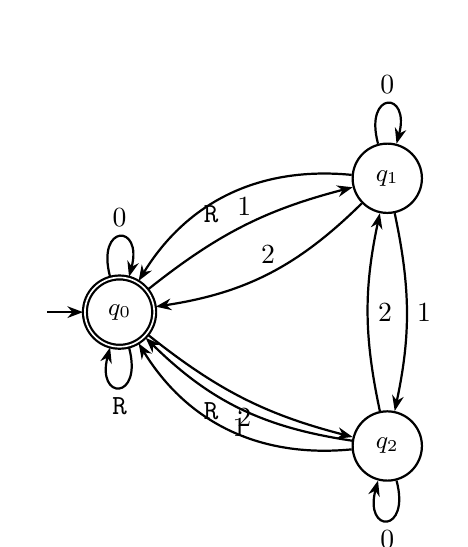
\begin{tikzpicture}[automaton]
  \node[state,initial,accepting] (q0) at (0,0) {$q_0$};
  \node[state] (q1) at (3.4,1.7) {$q_1$};
  \node[state] (q2) at (3.4,-1.7) {$q_2$};
  \path[->]
    (q0) edge[loop above] node{$0$} ()
         edge[bend left=12] node[above]{$1$} (q1)
         edge[bend right=12] node[below]{$2$} (q2)
    (q1) edge[loop above] node{$0$} ()
         edge[bend left=12] node[right]{$1$} (q2)
         edge[bend left=18] node[above]{$2$} (q0)
    (q2) edge[loop below] node{$0$} ()
         edge[bend left=18] node[below]{$1$} (q0)
         edge[bend left=12] node[right]{$2$} (q1)
    (q1) edge[bend right=32] node[below left]{\texttt{R}} (q0)
    (q2) edge[bend left=32] node[above left]{\texttt{R}} (q0)
    (q0) edge[loop below] node{\texttt{R}} ();
\end{tikzpicture}
\end{center}
Finite memory is enough because only the residue class of the sum matters.
\end{example}

\subsection{Designing finite automata}
Design principle:
\begin{itemize}
  \item You must be ready to accept or reject after every prefix.
  \item You do \emph{not} have infinite memory.
  \item Each state records exactly the information you still need about the
        prefix read so far.
\end{itemize}

\begin{example}[Odd number of $1$s]
$A=\set{w\in\set{0,1}^*:w\text{ has an odd number of }1\text{s}}$.
Remember only the parity of the number of $1$s.
\begin{center}
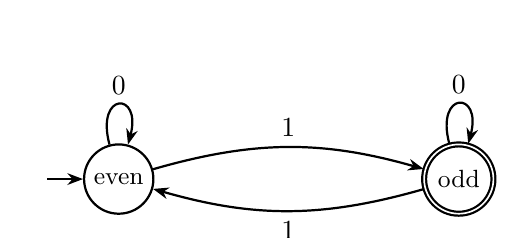
\begin{tikzpicture}[automaton,node distance=34mm]
  \node[state,initial] (even) {even};
  \node[state,accepting,right=of even] (odd) {odd};
  \path[->]
    (even) edge[loop above] node{$0$} ()
          edge[bend left=16] node[above]{$1$} (odd)
    (odd) edge[loop above] node{$0$} ()
         edge[bend left=16] node[below]{$1$} (even);
\end{tikzpicture}
\end{center}
\end{example}

\begin{example}[Substring $001$]
$A=\set{w\in\set{0,1}^*:w\text{ contains }001\text{ as a substring}}$.
States record the longest prefix of $001$ that is a suffix of the text so
far:
\[
  q_0:\text{nothing},\quad
  q_1:\text{suffix }0,\quad
  q_2:\text{suffix }00,\quad
  q_3:\text{already seen }001.
\]
\begin{center}
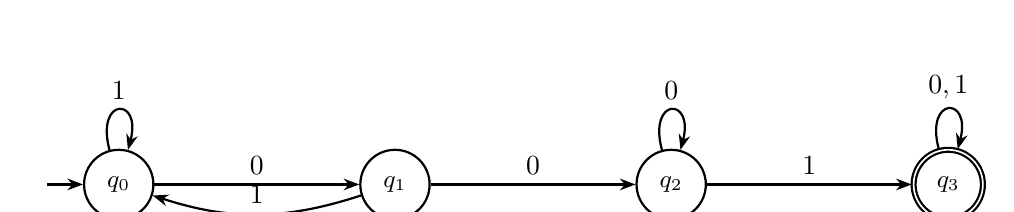
\begin{tikzpicture}[automaton,node distance=26mm]
  \node[state,initial] (q0) {$q_0$};
  \node[state,right=of q0] (q1) {$q_1$};
  \node[state,right=of q1] (q2) {$q_2$};
  \node[state,accepting,right=of q2] (q3) {$q_3$};
  \path[->]
    (q0) edge[loop above] node{$1$} ()
         edge node[above]{$0$} (q1)
    (q1) edge[bend left=18] node[above]{$1$} (q0)
         edge node[above]{$0$} (q2)
    (q2) edge[loop above] node{$0$} ()
         edge node[above]{$1$} (q3)
    (q3) edge[loop above] node{$0,1$} ();
\end{tikzpicture}
\end{center}
On a $0$ from $q_2$ we stay in $q_2$, because the suffix is still $00$.
\end{example}

\subsection{Formal definition of computation}
\begin{definition}[Computation of a DFA]
Let $M=(Q,\Sigma,\transition,q_0,F)$ and let $w=w_1w_2\cdots w_n$ with each
$w_i\in\Sigma$ (the case $n=0$ is $w=\eps$). Then $M$ \emph{accepts} $w$ if
there is a sequence of states $r_0,r_1,\ldots,r_n\in Q$ such that
\begin{enumerate}
  \item $r_0=q_0$;
  \item $\transition(r_i,w_{i+1})=r_{i+1}$ for $0\leq i\leq n-1$;
  \item $r_n\in F$.
\end{enumerate}
\end{definition}
Equivalently, extend $\transition$ to strings by
\[
  \transition^*(q,\eps)=q,\qquad
  \transition^*(q,wa)=\transition(\transition^*(q,w),a).
\]
Then $\lang{M}=\set{w\in\Sigma^*:\transition^*(q_0,w)\in F}$.

If $\transition(r_i,w_{i+1})=r_{i+1}$, we say that $M$ is in state $r_{i+1}$
after processing $w_1\cdots w_{i+1}$.

\begin{definition}[Regular language]
A language is \emph{regular} if some DFA recognizes it.
\end{definition}

\section{Regular operations and closure under union}

\subsection{The three regular operations}
Let $A$ and $B$ be languages, not necessarily over the same alphabet. If the
alphabets differ, replace both by $\Sigma_A\cup\Sigma_B$.

\begin{definition}[Regular operations]
\[
\begin{aligned}
  A\cup B
    &=\set{w:w\in A\text{ or }w\in B},\\
  A\concat B
    &=\set{xy:x\in A,\, y\in B},\\
  A^*
    &=\set{x_1x_2\cdots x_k:k\geq 0,\, x_i\in A}.
\end{aligned}
\]
By convention $A^0=\set{\eps}$, so $\eps\in A^*$ always, even if
$\eps\notin A$.
\end{definition}

\begin{example}
Let $A=\set{00,11}$ over $\set{0,1}$ and $B=\set{ab,ba}$ over $\set{a,b}$. Then
\[
\begin{aligned}
  A\cup B
    &=\set{00,11,ab,ba}
    &&\text{(alphabet }\set{0,1,a,b}\text{),}\\
  A\concat B
    &=\set{00ab,00ba,11ab,11ba},\\
  A^*
    &=\set{\eps,00,11,0000,0011,1100,1111,\ldots}.
\end{aligned}
\]
\end{example}

\begin{theorem}
Regular languages are closed under union, concatenation, and star.
\end{theorem}
The union case is proved with a product DFA. Concatenation and star need
nondeterminism; those constructions appear in Chapter~\ref{ch:nfa}.

\subsection{Closure under union: product construction}
\begin{theorem}[Union of regular languages]
If $A$ and $B$ are regular, then $A\cup B$ is regular.
\end{theorem}

\begin{proof}
If $A$ and $B$ use different alphabets $\Sigma_1$ and $\Sigma_2$, work over
$\Sigma=\Sigma_1\cup\Sigma_2$. Let
\[
  M_1=(Q_1,\Sigma,\transition_1,q_1,F_1),\qquad
  M_2=(Q_2,\Sigma,\transition_2,q_2,F_2)
\]
recognize $A$ and $B$. The idea is to run $M_1$ and $M_2$
\emph{simultaneously} on the same input.

Define the product DFA
\[
  M=(Q_1\times Q_2,\Sigma,\transition,(q_1,q_2),F),
\]
where
\[
  \transition\bigl((r,s),a\bigr)
    =\bigl(\transition_1(r,a),\transition_2(s,a)\bigr)
\]
and
\[
  F=\set{(r,s):r\in F_1\text{ or }s\in F_2}.
\]

\textbf{Claim.} $M$ accepts $w\in\Sigma^*$ if and only if $w\in A\cup B$.

\textbf{Subclaim.} For every $w\in\Sigma^*$, after reading $w$ the machine
$M_1$ is in state $r$, $M_2$ is in state $s$, if and only if $M$ is in state
$(r,s)$.

\textit{Proof of the subclaim, by induction on $|w|$.}
If $w=\eps$, then $M_1$ is in $q_1$, $M_2$ is in $q_2$, and $M$ is in
$(q_1,q_2)$.

Let $w=w'a$ with $|w'|=n-1$ and last symbol $a=w_n$. By the inductive
hypothesis, $M$ is in $(r,s)$ after $w'$ if and only if $M_1$ is in $r$ and
$M_2$ is in $s$. The next transitions are
\[
  \transition_1(r,a)=r',\qquad
  \transition_2(s,a)=s',\qquad
  \transition\bigl((r,s),a\bigr)=(r',s').
\]
Hence after $w$ the product is in $(r',s')$ if and only if $M_1$ is in $r'$
and $M_2$ is in $s'$.

\textit{Proof of the claim, assuming the subclaim.}
$M$ accepts $w$ if and only if, after $w$, it is in some $(r,s)\in F$, if and
only if $r\in F_1$ or $s\in F_2$, if and only if $M_1$ or $M_2$ accepts $w$,
if and only if $w\in A\cup B$.
\end{proof}

\begin{figure}[ht]
\centering
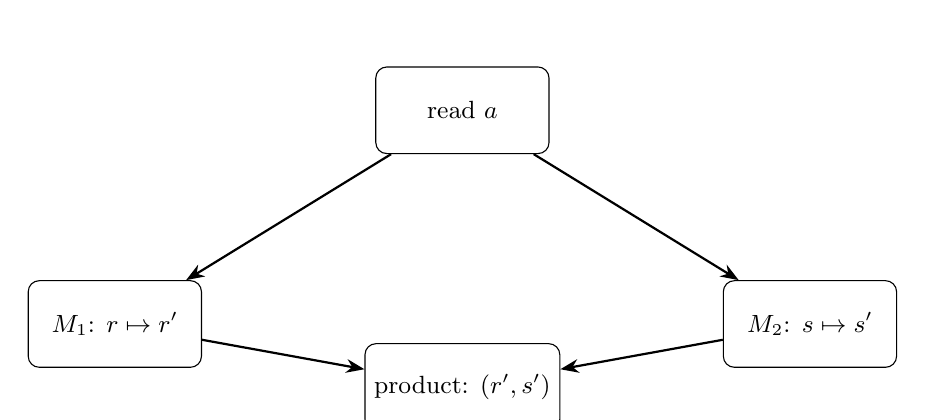
\begin{tikzpicture}[node distance=16mm and 22mm]
  \node[box] (in) {read $a$};
  \node[box,below left=of in] (m1) {$M_1$: $r\mapsto r'$};
  \node[box,below right=of in] (m2) {$M_2$: $s\mapsto s'$};
  \node[box,below=24mm of in] (p) {product: $(r',s')$};
  \draw[arrow] (in) -- (m1);
  \draw[arrow] (in) -- (m2);
  \draw[arrow] (m1) -- (p);
  \draw[arrow] (m2) -- (p);
\end{tikzpicture}
\caption{The product DFA stores both component states and updates them in lockstep.}
\end{figure}

\begin{exercise}
Let $M$ be a DFA over $\Sigma$ recognizing $A$. Construct a DFA for the
complement $\overline{A}=\Sigma^*\setminus A$ by swapping accept and
non-accept states. (Missing symbols of a larger alphabet should go to a
permanent rejecting sink.)
\end{exercise}

\subsection{Why concatenation is harder}
To recognize $A\concat B$ a deterministic machine would have to know, while
reading, where the $A$-prefix ends and the $B$-suffix begins. That cut-point
cannot in general be determined with finite memory. Therefore:
\begin{itemize}
  \item a single DFA product does not capture concatenation;
  \item we need \emph{nondeterminism}: the machine may guess the cut.
\end{itemize}

\section{Nondeterministic finite automata}
\label{ch:nfa}

\subsection{From DFA to NFA}
Nondeterminism captures guessing: at a step there may be
many legal next states. Every DFA is an NFA, but an NFA may have
\begin{itemize}
  \item zero, one, or several outgoing arrows for a given state and symbol;
  \item $\eps$-transitions that consume no input.
\end{itemize}

\textbf{Computation as splitting.} Whenever several moves are possible, the
machine splits into copies, one per choice. Each copy proceeds independently
and may split again. A copy with no legal move dies. The NFA accepts if
\emph{any} copy is in an accept state after the input is fully read.

An $\eps$-transition from $q$ to $r$ immediately starts an extra copy in $r$
without reading a symbol. Think of threads or \texttt{fork}.

\begin{example}[An NFA with $\eps$-moves]
\begin{center}
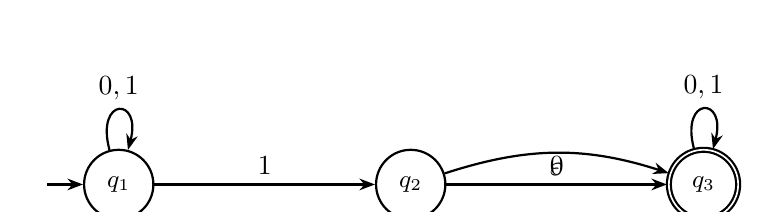
\begin{tikzpicture}[automaton,node distance=28mm]
  \node[state,initial] (q1) {$q_1$};
  \node[state,right=of q1] (q2) {$q_2$};
  \node[state,accepting,right=of q2] (q3) {$q_3$};
  \path[->]
    (q1) edge[loop above] node{$0,1$} ()
         edge node[above]{$1$} (q2)
    (q2) edge node[above]{$0$} (q3)
         edge[bend left=18] node[below]{$\eps$} (q3)
    (q3) edge[loop above] node{$0,1$} ();
\end{tikzpicture}
\end{center}
On input $010110$ some thread reaches an accept state, so the NFA accepts.
\end{example}

\begin{exercise}
For every NFA $N$, construct an equivalent NFA $N'$ with no $\varepsilon$-transitions.
(Replace each $\transition(q,a)$ by the $\varepsilon$-closure of that set; start
from the $\varepsilon$-closure of $q_0$.)
\end{exercise}

\begin{exercise}
Determine the language of the NFA in the previous example on input $010110$.
\end{exercise}

\subsection{Why nondeterminism helps}
\begin{itemize}
  \item Some languages have a tiny NFA but an exponentially larger DFA.
  \item Nondeterminism is a useful preview of later models (NPDA, NTMs).
\end{itemize}

\begin{example}[Third symbol from the end is $1$]
\[
  A=\set{w\in\set{0,1}^*: \text{the third symbol from the end of }w\text{ is }1}.
\]
$01001$ is rejected; $010100$ is accepted. An NFA guesses which $1$ is the
third-from-last symbol and then verifies the last two symbols:
\begin{center}
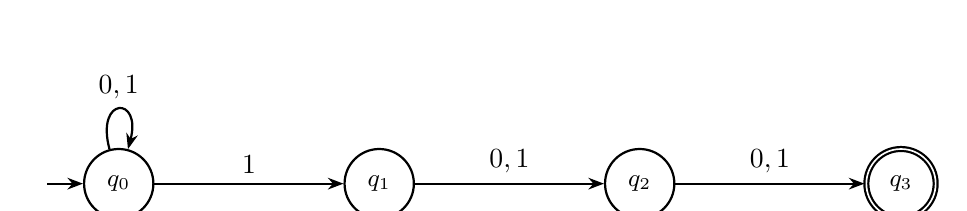
\begin{tikzpicture}[automaton,node distance=24mm]
  \node[state,initial] (q0) {$q_0$};
  \node[state,right=of q0] (q1) {$q_1$};
  \node[state,right=of q1] (q2) {$q_2$};
  \node[state,accepting,right=of q2] (q3) {$q_3$};
  \path[->]
    (q0) edge[loop above] node{$0,1$} ()
         edge node[above]{$1$} (q1)
    (q1) edge node[above]{$0,1$} (q2)
    (q2) edge node[above]{$0,1$} (q3);
\end{tikzpicture}
\end{center}
Any DFA for $A$ needs at least $8=2^3$ states: it must remember the last three
symbols.
\end{example}

\subsection{Formal definition of an NFA}
\begin{definition}[NFA]
A \emph{nondeterministic finite automaton} is a $5$-tuple
\[
  N=(Q,\Sigma,\transition,q_0,F)
\]
where $Q$ is a finite set of states, $\Sigma$ is a finite alphabet,
\[
  \transition:Q\times\Sigma_\eps\to\powerset{Q},
  \qquad \Sigma_\eps=\Sigma\cup\set{\eps},
\]
$q_0\in Q$ is the start state, and $F\subseteq Q$ is the set of accept
states. Here $\powerset{Q}$ is the power set of $Q$.
\end{definition}
A DFA is the special case in which $\transition(q,a)$ is always a singleton,
$\transition(q,\eps)=\varnothing$, and there is exactly one outgoing $a$-edge
from each state.

\begin{definition}[Computation of an NFA]
Let $N=(Q,\Sigma,\transition,q_0,F)$ and $w\in\Sigma^*$. Write $w=y_1y_2\cdots y_m$
with each $y_i\in\Sigma_\eps$ (so $\eps$-symbols may be inserted). Then $N$
accepts $w$ if there is a sequence of states $r_0,r_1,\ldots,r_m$ such that
\begin{enumerate}
  \item $r_0=q_0$;
  \item $r_{i+1}\in\transition(r_i,y_{i+1})$ for $0\leq i\leq m-1$;
  \item $r_m\in F$.
\end{enumerate}
\end{definition}

\subsection{Equivalence of NFAs and DFAs}
\begin{definition}
Two automata $M_1$ and $M_2$ (DFA or NFA) are \emph{equivalent} if
$\lang{M_1}=\lang{M_2}$.
\end{definition}

\begin{theorem}[Subset construction]
For every NFA $N$ there is an equivalent DFA $M$.
\end{theorem}

\begin{proof}[Construction]
Let $N=(Q,\Sigma,\transition,q_0,F)$. First ignore $\eps$-moves. Define
\[
  M=\bigl(\powerset{Q},\Sigma,\Delta,\set{q_0},F'\bigr),
\]
where
\[
  \Delta(R,a)=\bigcup_{r\in R}\transition(r,a)
  =\set{q:q\in\transition(r,a)\text{ for some }r\in R}
\]
and
\[
  F'=\set{R\subseteq Q:R\cap F\neq\varnothing}.
\]
The DFA state after reading $w$ is exactly the set of NFA states reachable
on $w$. It is accepting if and only if some reachable NFA state is accepting.

\textbf{$\eps$-moves.} For $R\subseteq Q$ let $E(R)$ be the
\emph{$\eps$-closure}: all states reachable from $R$ by zero or more
$\eps$-moves. Then set
\[
  \Delta(R,a)=E\!\Bigl(\bigcup_{r\in R}\transition(r,a)\Bigr),
  \qquad
  \text{start state }=E(\set{q_0}).
\]
Correctness is by induction on $|w|$, as in the product-construction proof.
\end{proof}

\begin{corollary}
A language is regular if and only if it is recognized by an NFA (with or
without $\eps$-moves).
\end{corollary}

\begin{exercise}
Carry out the subset construction on the third-from-last NFA.
\end{exercise}

\subsection{NFA proofs of the remaining closure properties}
With $\eps$-NFAs the constructions are diagrams rather than products.

\begin{theorem}
Regular languages are closed under union, concatenation, and star.
\end{theorem}

\begin{proof}[NFA constructions]
Let $N_1$ and $N_2$ recognize $A$ and $B$.

\textbf{Union.} Add a new start state $q_0$ with $\eps$-edges to the old start
states of $N_1$ and $N_2$. Accepting states are the old accepting states of both
machines.

\textbf{Concatenation.} Put an $\eps$-edge from every accept state of $N_1$ to
the start state of $N_2$. Keep only $N_2$'s accept states. The new start state
is $N_1$'s start state.

\textbf{Star.} Add a new start state $q_0$ that is also accepting, with an
$\eps$-edge to the old start. From every old accept state, add an $\eps$-edge
back to the old start (and to $q_0$ if desired). Then $\eps$ is accepted, and
any concatenation of words from $A$ can be guessed as a sequence of loops.
\end{proof}

Combined with the subset construction they complete the proof that regular
languages are closed under the three regular operations.

\begin{center}
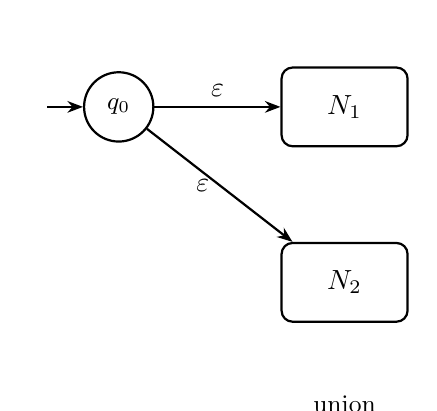
\begin{tikzpicture}[automaton,node distance=16mm]
  \node[state,initial] (u) {$q_0$};
  \node[draw,rounded corners,minimum width=16mm,minimum height=10mm,right=of u] (n1) {$N_1$};
  \node[draw,rounded corners,minimum width=16mm,minimum height=10mm,below=12mm of n1] (n2) {$N_2$};
  \path[->]
    (u) edge node[above]{$\eps$} (n1)
    (u) edge node[left]{$\eps$} (n2);
  \node[below=8mm of n2,font=\small] {union};
\end{tikzpicture}
\hspace{6mm}
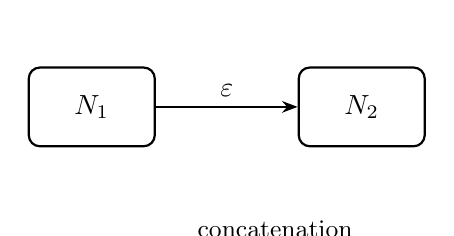
\begin{tikzpicture}[automaton,node distance=18mm]
  \node[draw,rounded corners,minimum width=16mm,minimum height=10mm] (a) {$N_1$};
  \node[draw,rounded corners,minimum width=16mm,minimum height=10mm,right=of a] (b) {$N_2$};
  \path[->] (a) edge node[above]{$\eps$} (b);
  \node[below=10mm of a] {};
  \node[below=8mm of b,xshift=-11mm,font=\small] {concatenation};
\end{tikzpicture}
\hspace{6mm}
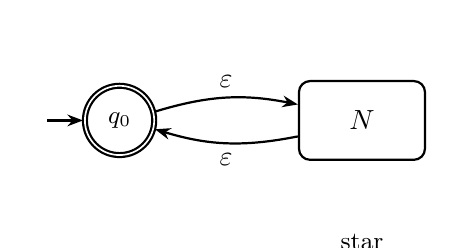
\begin{tikzpicture}[automaton,node distance=18mm]
  \node[state,initial,accepting] (s) {$q_0$};
  \node[draw,rounded corners,minimum width=16mm,minimum height=10mm,right=of s] (n) {$N$};
  \path[->]
    (s) edge[bend left=14] node[above]{$\eps$} (n)
    (n) edge[bend left=14] node[below]{$\eps$} (s);
  \node[below=8mm of n,font=\small] {star};
\end{tikzpicture}
\end{center}

\section{Regular expressions and Kleene's theorem}

\subsection{Regular expressions as shorthand}
A regular expression is a compact description of a regular
language. Examples over $\Sigma=\set{0,1}$:
\[
\begin{aligned}
  0^*10^*
    &=\set{w:w\text{ contains exactly one }1},\\
  \Sigma^*1
    &=\set{w:w\text{ ends with }1},\\
  0\Sigma^*\cup\Sigma^*1
    &=\set{w:w\text{ starts with }0\text{ or ends with }1},\\
  (0\cup 1)^*001(0\cup 1)^*
    &=\set{w:w\text{ contains }001\text{ as a substring}},\\
  (00)^*
    &=\set{w:|w|\text{ is even and }w\in 0^*},\\
  (0\cup 1)(0\cup 1)
    &=\set{w:|w|=2},\\
  (0\cup\varepsilon)1^*
    &=\set{0^i1^k:i\in\set{0,1},\,k\geq 0},\\
  0(0\cup 1)^*0\cup 1(0\cup 1)^*1\cup 0\cup 1
    &=\set{w:w\text{ starts and ends with the same symbol}}.
\end{aligned}
\]
Useful identities include
\[
  A\cup\varnothing=A,\qquad
  A\concat\varnothing=\varnothing,\qquad
  A\concat\set{\eps}=A,\qquad
  A\cup\set{\eps}=A\text{ if and only if }\eps\in A.
\]
$R\cup\eps$ need not equal $R$ unless $\eps$ is already in $\lang{R}$.

\textbf{Operator precedence} (highest to lowest): star, then concatenation, then
union. Use parentheses to override.

\subsection{Formal definition}
\begin{definition}[Regular expression]
$R$ is a regular expression over $\Sigma$ if it has one of the forms
\begin{enumerate}
  \item $R=a$ for some $a\in\Sigma$;
  \item $R=\eps$;
  \item $R=\varnothing$;
  \item $R=(R_1\cup R_2)$;
  \item $R=(R_1R_2)$;
  \item $R=(R_1^*)$;
\end{enumerate}
where $R_1$ and $R_2$ are regular expressions. The language $\lang{R}$ is
defined inductively:
\[
\begin{aligned}
  \lang{a}&=\set{a},&
  \lang{\eps}&=\set{\eps},&
  \lang{\varnothing}&=\varnothing,\\
  \lang{R_1\cup R_2}&=\lang{R_1}\cup\lang{R_2},&
  \lang{R_1R_2}&=\lang{R_1}\concat\lang{R_2},&
  \lang{R_1^*}&=\lang{R_1}^*.
\end{aligned}
\]
\end{definition}
Write $R^+$ for $RR^*$, which excludes $\eps$ unless $\eps\in\lang{R}$. Then
$R^*\equiv R^+\cup\set{\eps}$.

\subsection{Kleene's theorem}
\begin{theorem}[Kleene]
A language is regular if and only if some regular expression describes it.
\end{theorem}
The two directions are the next two lemmas.

\begin{lemma}[Expression $\Rightarrow$ automaton]
If a language is described by a regular expression, then it is regular.
\end{lemma}

\begin{proof}
Let $R$ be a regular expression. Induct on the structure of $R$.
\begin{enumerate}
  \item $R=a$: a two-state NFA with a single $a$-edge from start to accept.
  \item $R=\eps$: a single accepting start state and no edges (or an
        $\eps$-edge to an accept state).
  \item $R=\varnothing$: a start state that is not accepting, and no edges.
  \item $R=R_1\cup R_2$, $R=R_1R_2$, $R=R_1^*$: apply the NFA constructions of
        Chapter~\ref{ch:nfa} to the machines given by the inductive hypothesis.
\end{enumerate}
\end{proof}

\begin{exercise}
Build, by the inductive method, an NFA for $(ab\cup a)^*$ and compare it with
an NFA for $(ab^*\cup a^*)$. They are not the same language.
\end{exercise}

\subsection{Generalized NFAs}
\begin{lemma}[Automaton $\Rightarrow$ expression]
If a language is regular, then it is described by a regular expression.
\end{lemma}

\begin{proof}[Idea]
Convert a DFA to a \emph{generalized NFA} (GNFA), then eliminate states until
a single regular-expression label remains.

A GNFA has regular expressions (not just symbols) as edge labels, and satisfies:
\begin{enumerate}
  \item a unique start state with edges to every other state, and no incoming
        edges;
  \item a unique accept state with edges from every other state, and no
        outgoing edges;
  \item for every pair of non-start, non-accept states (including a state and
        itself), edges in both directions.
\end{enumerate}
Missing edges are labelled $\varnothing$.

\textbf{DFA to GNFA.} Add a new start state with an $\eps$-edge to the old
start. Add a new unique accept state with $\eps$-edges from every old accept
state. Combine multiple labels $R,S$ on the same pair of states into
$R\cup S$. Add $\varnothing$ labels where no edge existed.

\begin{definition}[GNFA]
A GNFA is a $5$-tuple $(Q,\Sigma,\transition,q_{\mathrm{start}},q_{\mathrm{accept}})$
where
\[
  \transition:
    \bigl(Q\setminus\set{q_{\mathrm{accept}}}\bigr)
    \times
    \bigl(Q\setminus\set{q_{\mathrm{start}}}\bigr)
    \to \mathcal{R}
\]
and $\mathcal{R}$ is the set of regular expressions over $\Sigma$. It accepts $w$
if $w$ can be broken into pieces matching the labels of some path from
$q_{\mathrm{start}}$ to $q_{\mathrm{accept}}$.
\end{definition}

\begin{center}
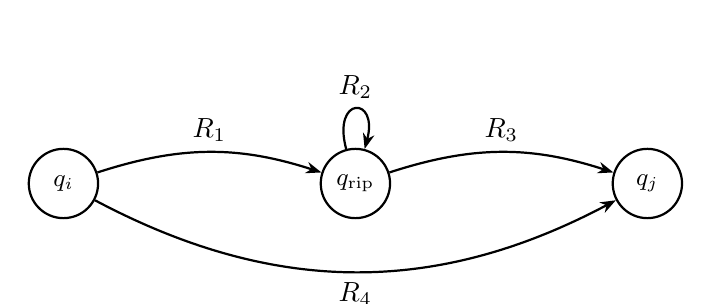
\begin{tikzpicture}[automaton,node distance=28mm]
  \node[state] (qi) {$q_i$};
  \node[state,right=of qi] (rip) {$q_{\mathrm{rip}}$};
  \node[state,right=of rip] (qj) {$q_j$};
  \path[->]
    (qi) edge[bend left=18] node[above]{$R_1$} (rip)
    (rip) edge[loop above] node{$R_2$} ()
    (rip) edge[bend left=18] node[above]{$R_3$} (qj)
    (qi) edge[bend right=28] node[below]{$R_4$} (qj);
\end{tikzpicture}
\end{center}
After removing $q_{\mathrm{rip}}$, the direct label $q_i\to q_j$ becomes
$R_4\cup R_1(R_2)^*R_3$.

\textbf{State elimination.} While more than two states remain, pick a state
$q_{\mathrm{rip}}\notin\set{q_{\mathrm{start}},q_{\mathrm{accept}}}$ and remove
it. For every remaining $q_i,q_j$ (not the accept as source, not the start as
target), replace the $q_i\to q_j$ label $R_4$ by
\[
  R_4\cup\bigl(R_1(R_2)^*R_3\bigr),
\]
where $R_1$ labels $q_i\to q_{\mathrm{rip}}$, $R_2$ labels the loop at
$q_{\mathrm{rip}}$, $R_3$ labels $q_{\mathrm{rip}}\to q_j$, and $R_4$ is the old
direct label $q_i\to q_j$.

When two states remain, the label of the unique edge
$q_{\mathrm{start}}\to q_{\mathrm{accept}}$ is the desired expression.

Correctness is by induction on the number $k$ of states of the GNFA. The base
$k=2$ is immediate. The inductive step: any path
that used $q_{\mathrm{rip}}$ is accounted for by $R_1(R_2)^*R_3$, and paths
that never used it are accounted for by $R_4$.
\end{proof}

\begin{exercise}
Convert the odd-parity DFA and the substring-$001$ DFA to regular
expressions by state elimination.
\end{exercise}

\section{Nonregular languages and the pumping lemma}

\subsection{Languages that look nonregular}
We now know
\[
  \text{DFA}\;\equiv\;\text{NFA}\;\equiv\;\text{regular expressions}.
\]
Candidate nonregular languages:
\[
\begin{aligned}
  B&=\set{0^n1^n:n\geq 0},\\
  C&=\set{w\in\set{0,1}^*:w\text{ has equally many }0\text{s and }1\text{s}},\\
  F&=\set{ww:w\in\set{0,1}^*}.
\end{aligned}
\]
$B$ seems to require remembering how many $0$s have been seen. Finite memory
cannot do that for arbitrary $n$.

\begin{exercise}
Let $D$ be the language of strings over $\set{0,1}$ with equally many
occurrences of the substrings $01$ and $10$. Show that $D$ is regular.
(The language depends only on the first and last symbols.)
\end{exercise}

\begin{exercise}
Every finite language is regular. (Build a tree-like DFA, or a regular
expression that is a finite union of concrete words.)
\end{exercise}

\subsection{The pumping lemma}
If a DFA has $p$ states and a string of length at least $p$ is accepted, then
in the run some state repeats. The substring that takes the machine around
that loop can be repeated any number of times.

\begin{lemma}[Pumping lemma for regular languages]
If $A$ is regular, then there exists a pumping length $p\geq 1$ such that every
$s\in A$ with $|s|\geq p$ can be written $s=xyz$ satisfying
\begin{enumerate}
  \item $xy^iz\in A$ for every $i\geq 0$;
  \item $|y|>0$;
  \item $|xy|\leq p$.
\end{enumerate}
The strings $x$ and $z$ are allowed to be $\eps$.
\end{lemma}

\begin{proof}
Let $M=(Q,\Sigma,\transition,q_0,F)$ recognize $A$, and set $p=|Q|$. Let
$s=s_1s_2\cdots s_n\in A$ with $n\geq p$. Let $r_0,r_1,\ldots,r_n$ be the
states visited, so $r_0=q_0$, $r_{j}=\transition(r_{j-1},s_j)$, and
$r_n\in F$. The prefix sequence $r_0,\ldots,r_p$ has length $p+1$, so two of
these states coincide: take the first repeated state, at positions $i<j$
with $0\leq i<j\leq p$. Set
\[
  x=s_1\cdots s_i,\qquad
  y=s_{i+1}\cdots s_j,\qquad
  z=s_{j+1}\cdots s_n.
\]
Then $y$ takes $M$ from that state back to itself, so $xy^iz$ is accepted for
every $i\geq 0$. Also $|y|=j-i\geq 1$ and $|xy|=j\leq p$.
\end{proof}

\begin{center}
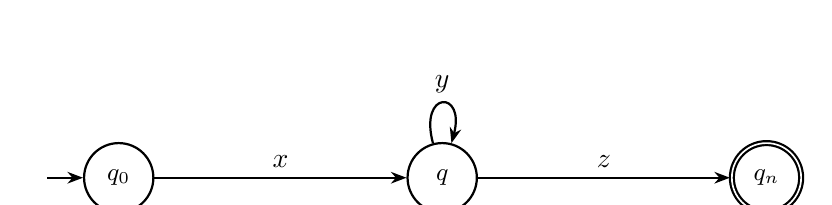
\begin{tikzpicture}[automaton,node distance=32mm]
  \node[state,initial] (q0) {$q_0$};
  \node[state,right=of q0] (qi) {$q$};
  \node[state,accepting,right=of qi] (qn) {$q_n$};
  \path[->]
    (q0) edge node[above]{$x$} (qi)
    (qi) edge[loop above] node{$y$} ()
    (qi) edge node[above]{$z$} (qn);
\end{tikzpicture}
\end{center}
The repeated state is $q=q_i=q_j$. Pumping $y$ stays in $q$ and still reaches
an accept state.

\subsection{How to prove a language is not regular}
Quantifier order:
\[
  \text{assume regular}
  \;\to\;
  \text{obtain }p
  \;\to\;
  \text{choose }s
  \;\to\;
  \text{defeat every }xyz
  \;\to\;
  \text{choose }i.
\]
You do not get to pick the decomposition; the adversary does. You must show
that \emph{every} $xyz$ obeying $|xy|\leq p$ and $|y|\geq 1$ fails for some
$i$.

\begin{example}[$B=\set{0^n1^n:n\geq 0}$]
Suppose $B$ is regular with pumping length $p$. Choose $s=0^p1^p$. Then
$|s|\geq p$. For any decomposition $s=xyz$ with $|xy|\leq p$ and $|y|\geq 1$,
the string $y$ lies entirely in the $0$s, so $y=0^k$ with $k\geq 1$. Pumping
with $i=0$ (or $i=2$) changes the number of $0$s but not the number of $1$s,
so $xy^iz\notin B$. Contradiction.
\end{example}

\begin{example}[$C=\set{w:\text{equal number of }0\text{s and }1\text{s}}$]
The same $s=0^p1^p$ works: $y$ is again a nonempty block of $0$s, and
$xy^2z$ has more $0$s than $1$s. (Choosing $s=(01)^p$ does \emph{not} work:
$y$ might be $01$, which pumps inside $C$.)
\end{example}

\begin{example}[$F=\set{ww:w\in\set{0,1}^*}$]
Take $s=0^p10^p1$. Then $|s|\geq p$. If $y$ lies in the first block of $0$s,
pumping breaks the two-copy structure. The Myhill--Nerode argument in the
next section is cleaner.
\end{example}

\begin{example}[$E=\set{0^i1^j:i\neq j}$]
A standard trick: if $E$ were regular then
$B=\overline{E}\cap 0^*1^*$ would be regular, but $B=\set{0^n1^n:n\geq 0}$.
Direct pumping on $0^{p}1^{p!+p}$ is another option (pumping $i=0$ is not
enough; the factorial gap prevents accidental equality).
\end{example}

\begin{exercise}
Show that $\set{1^{n^2}:n\geq 0}$ is not regular.
\end{exercise}

\section{DFA minimization and the Myhill--Nerode theorem}

\subsection{Equivalent versus distinguishable states}
Let $M=(Q,\Sigma,\transition,q_0,F)$ be a DFA. Write
$\transition^*(q,x)$ for the state reached from $q$ on $x$.

\begin{definition}[Distinguishable states]
States $p,q\in Q$ are \emph{equivalent} if
\[
  \forall x\in\Sigma^*:\quad
  \bigl(\transition^*(p,x)\in F
        \iff
        \transition^*(q,x)\in F\bigr).
\]
Otherwise they are \emph{distinguishable}: some witness $x$ sends exactly one
of them into $F$. Equivalently, once the machine is in $p$ versus $q$, no
future input can tell the two situations apart if and only if $p$ and $q$
are equivalent.
\end{definition}
Accepting and non-accepting states are always distinguishable (witness $\eps$).

\subsection{The table-filling algorithm}
\begin{algorithm}[Table filling]
\begin{enumerate}
  \item Remove unreachable states by BFS/DFS from $q_0$.
  \item Make a table of unordered pairs $\set{p,q}$ with $p\neq q$.
  \item Mark every pair in which exactly one state is accepting.
  \item Repeat: if an unmarked pair $\set{p,q}$ has, for some $a\in\Sigma$,
        the pair $\set{\transition(p,a),\transition(q,a)}$ already marked, then
        mark $\set{p,q}$. (If $\transition(p,a)=r$ and $\transition(q,a)=s$ are
        distinguishable, then $ax$ distinguishes $p$ and $q$ whenever $x$
        distinguishes $r$ and $s$.)
  \item Stop when a pass marks nothing new. Unmarked pairs are equivalent.
        Merge equivalent states.
\end{enumerate}
\end{algorithm}

\begin{theorem}[Correctness of table filling]
A pair is marked if and only if it is distinguishable.
\end{theorem}

\begin{proof}
($\Rightarrow$) Induction on the iteration in which the pair is marked. Pairs
marked in step~3 are distinguished by $\eps$. If $\set{p,q}$ is marked because
$\set{\transition(p,a),\transition(q,a)}$ was already marked, the inductive
hypothesis gives a witness $x$ for the successors, so $ax$ witnesses
$\set{p,q}$.

($\Leftarrow$) Induction on the length of a shortest distinguishing word.
If $|x|=0$, then $x=\eps$ and the pair is marked in step~3. If
$x=ax'$ with $|x|=k+1$, then $x'$ distinguishes
$r=\transition(p,a)$ and $s=\transition(q,a)$ and has length $k$, so
$\set{r,s}$ is already marked by the inductive hypothesis. Step~4 therefore
marks $\set{p,q}$.
\end{proof}

The relation ``unmarked'' is an equivalence relation on the (reachable) states.
The \emph{minimal DFA} has those equivalence classes as states:
\[
  M'=\bigl(Q/{\sim},\;\Sigma,\;\transition',\;[q_0],\;
           \set{[q]:q\in F}\bigr),
  \qquad
  \transition'([q],a)=[\transition(q,a)].
\]
$\transition'$ is well-defined: if $q\sim r$ but
$\transition(q,a)\not\sim\transition(r,a)$, then some $x$ distinguishes the
successors, so $ax$ distinguishes $q$ and $r$. An accept state and a reject
state never lie in the same class.

\begin{theorem}
$\lang{M'}=\lang{M}$, and $M'$ has the fewest states among all DFAs equivalent
to $M$.
\end{theorem}

\begin{proof}[Sketch]
A run of $M$ on $w$ visits $q_0,q_1,\ldots,q_n$; the corresponding run of $M'$
visits $[q_0],[q_1],\ldots,[q_n]$. The last class is accepting if and only if
$q_n\in F$, so the languages coincide.

If some equivalent DFA $N$ had fewer states than $M'$, then two distinct
classes $[p]$ and $[q]$ of $M'$ would map to the same state of $N$. A witness
that distinguishes $p$ and $q$ would then distinguish that state of $N$ from
itself, which is impossible. Hence $M'$ is minimal.
\end{proof}

\begin{example}[Table filling on a four-state DFA]
Let $Q=\set{1,2,3,4}$ with $1$ start, $F=\set{3,4}$, and
\[
\begin{array}{c|cc}
 & 0 & 1\\
\hline
1 & 2 & 3\\
2 & 1 & 4\\
3 & 4 & 3\\
4 & 3 & 4
\end{array}
\]
Pairs mixing $\set{1,2}$ with $\set{3,4}$ are marked immediately. Then
$\transition(1,1)=3$ and $\transition(2,1)=4$ are both accepting, while
$\transition(3,0)=4$ and $\transition(4,0)=3$ stay unmarked. The unmarked
pairs are $\set{1,2}$ and $\set{3,4}$. The minimal DFA therefore has two
states: $\set{1,2}$ (reject) and $\set{3,4}$ (accept).
\end{example}

\subsection{Equivalence of strings}
The same idea, lifted from states to strings, is independent of any particular
machine.

\begin{definition}[Myhill--Nerode relation]
For a language $A\subseteq\Sigma^*$ define
\[
  x\equiv_A y
  \quad\Longleftrightarrow\quad
  \forall z\in\Sigma^*:\;
  (xz\in A\iff yz\in A).
\]
Strings $x,y$ are equivalent when no future $z$ can tell them apart; they
represent the same knowledge about $A$.
\end{definition}

\begin{example}[Strings ending in $1$]
Let $L=\set{w:w\text{ ends in }1}$. Then
$00\equiv_L 000\equiv_L 1000$ (all ``last symbol is $0$''), while
$1$, $01$, $001$ are another class. Two classes: last bit $0$ versus last
bit $1$.

For $A=\set{w:w\text{ ends in }00}$ there are three relevant classes:
ends in $00$; ends in $1$ (or is $\eps$ / ends in a $1$ not covered); ends
in a single $0$ not already forming the suffix $00$.
\end{example}

\subsection{Myhill--Nerode theorem}
\begin{theorem}[Myhill--Nerode]
The following are equivalent for $A\subseteq\Sigma^*$.
\begin{enumerate}
  \item $A$ is regular.
  \item $\equiv_A$ has finitely many equivalence classes.
\end{enumerate}
Moreover, the number of classes equals the number of states in the unique
(up to renaming) minimal DFA for $A$.
\end{theorem}

\begin{proof}
($\Rightarrow$) Let $M=(Q,\Sigma,\transition,q_0,F)$ recognize $A$. If
$\transition^*(q_0,x)=\transition^*(q_0,y)$, then $x\equiv_A y$, because
every continuation $z$ leads both strings to the same state. Contrapositively,
distinguishable strings go to different states. Hence the number of classes is
at most $|Q|$, which is finite.

($\Leftarrow$) Let the classes of $\equiv_A$ be the states of a DFA
\[
  M=\bigl(\set{[x]:x\in\Sigma^*},\;
          \Sigma,\;
          \transition,\;
          [\eps],\;
          \set{[x]:x\in A}\bigr),
\]
where $\transition([x],a)=[xa]$. This is well-defined by right-invariance of
$\equiv_A$: if $x\equiv_A y$ then $xa\equiv_A ya$.

\textbf{Claim.} $\transition^*([\eps],w)=[w]$ for every $w$. By induction on
$|w|$: the base is $[\eps]$; if the claim holds for $w$ then
\[
  \transition^*([\eps],wa)
    =\transition\bigl(\transition^*([\eps],w),a\bigr)
    =\transition([w],a)=[wa].
\]
Hence $M$ accepts $w$ if and only if $[w]$ is accepting if and only if
$w\in A$.

The construction uses exactly one state per class, so it is minimal. It
matches the table-filling DFA: two reachable states $p=\transition^*(q_0,x)$
and $q=\transition^*(q_0,y)$ are equivalent if and only if $x\equiv_A y$.
\end{proof}

\section{Context-free grammars}

\subsection{From \texorpdfstring{$0^n1^n$}{0n1n} to grammars}
The language $A=\set{0^n1^n:n\geq 0}$ is not regular, but it is generated by
recursively inserting $01$ in the middle:
\[
  S\to 0S1\mid\eps.
\]
A derivation of $0011$:
\[
  S\Rightarrow 0S1\Rightarrow 00S11\Rightarrow 00\eps 11=0011.
\]

\begin{exercise}
What context-free grammar generates (a simplified abstraction of) programs
in C? Typical answer: a grammar for nested blocks, declarations, and
balanced braces, not the full language of C.
\end{exercise}

\subsection{Formal definition}
\begin{definition}[Context-free grammar]
A \emph{context-free grammar} is a $4$-tuple $G=(V,\Sigma,R,S)$ where
\begin{enumerate}
  \item $V$ is a finite set of \emph{variables} (nonterminals);
  \item $\Sigma$ is a finite set of \emph{terminals}, $V\cap\Sigma=\varnothing$;
  \item $R$ is a finite set of \emph{rules} $A\to\alpha$ with $A\in V$ and
        $\alpha\in(V\cup\Sigma)^*$;
  \item $S\in V$ is the start variable.
\end{enumerate}
\end{definition}

If $u,v,w\in(V\cup\Sigma)^*$ and $A\to w$ is a rule, we say $uAv$
\emph{yields} $uwv$ and write $uAv\Rightarrow uwv$. We write $u\Rightarrow^* v$
if $u=v$ or there is a sequence $u=u_1\Rightarrow u_2\Rightarrow\cdots\Rightarrow u_k=v$.

The language of $G$ is
\[
  \lang{G}=\set{w\in\Sigma^*:S\Rightarrow^* w}.
\]
A string $w\in(V\cup\Sigma)^*$ with $S\Rightarrow^* w$ is a \emph{sentential
form}. A sentential form consisting only of terminals is a \emph{sentence}.

\textbf{Convention.} We often write only the rules. Variables are the symbols
that appear on the left of some rule; terminals are the remaining symbols;
the start variable is the left-hand side of the first rule.

\begin{example}
$G=(\set{S},\set{0,1},R,S)$ with $R=\set{S\to 0S1,\,S\to\eps}$. Then
\[
  S\Rightarrow 0S1\Rightarrow 00S11\Rightarrow 0011,
\]
so $0011\in\lang{G}$. Also $S\Rightarrow\eps$, and
$S\Rightarrow 0S1\Rightarrow 01$.
\end{example}

\begin{example}[Balanced parentheses]
$S\to(S)\,|\,SS\,|\,\eps$ generates the Dyck language of balanced parentheses.
Sample derivations:
\[
  S\Rightarrow(S)\Rightarrow(),
  \qquad
  S\Rightarrow SS\Rightarrow(S)S\Rightarrow()S\Rightarrow()(S)\Rightarrow()().
\]
\end{example}

\subsection{Leftmost and rightmost derivations}
If a right-hand side contains several variables, many substitution orders are
possible.

\begin{example}
$S\to AB$, $A\to aA\mid a$, $B\to bB\mid b$. Then $aabbb\in\lang{G}$.
A leftmost derivation always replaces the leftmost variable:
\[
  S\Rightarrow AB\Rightarrow aAB\Rightarrow aaB\Rightarrow aabB\Rightarrow aabbB\Rightarrow aabbb.
\]
A rightmost derivation:
\[
  S\Rightarrow AB\Rightarrow AbB\Rightarrow AbbB\Rightarrow Abbb\Rightarrow aAbbb\Rightarrow aabbb.
\]
\end{example}

\begin{definition}
A derivation is \emph{leftmost} (resp.\ \emph{rightmost}) if at every step the
leftmost (resp.\ rightmost) variable is replaced.
\end{definition}

A grammar is \emph{generating} if it has no dead rules that can never produce
a terminal string.

Regular languages are exactly the languages of right-linear grammars.
Given a DFA $M=(Q,\Sigma,\transition,q_0,F)$ with $Q=\set{q_0,\ldots,q_m}$,
take variables $V=Q$, start symbol $q_0$, and rules
\[
  q_i\to a\,q_j
  \quad\text{whenever}\quad
  \transition(q_i,a)=q_j,
  \qquad
  q_i\to\eps
  \quad\text{whenever}\quad
  q_i\in F.
\]
Then $\lang{G}=\lang{M}$. The converse (right-linear grammar to NFA) is the
same picture read backwards.

\subsection{Parse trees}
\begin{definition}[Parse tree]
A parse tree for a derivation in $G$ satisfies:
\begin{enumerate}
  \item the root is the start variable;
  \item every internal node is a variable $A$; if $A\to X_1\cdots X_k$ is the
        rule used, the children of $A$ are $X_1,\ldots,X_k$ in order
        ($k=0$ is an $\eps$-child);
  \item leaves are terminals (or $\eps$), and reading them left to right gives
        the derived string.
\end{enumerate}
\end{definition}
A derivation records the \emph{order} of substitutions; a parse tree records
the \emph{structure}. Leftmost and rightmost derivations of the same parse tree
describe the same nesting.

\begin{example}
For $S\to 0S1\mid\eps$ the parse tree of $0011$ is
\begin{center}
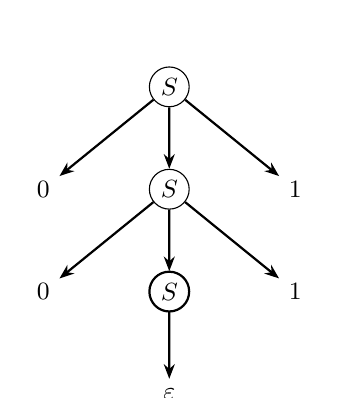
\begin{tikzpicture}[
  level distance=13mm,
  sibling distance=16mm,
  every node/.style={font=\small},
  edge from parent/.style={draw,-{Stealth[scale=0.8]},thick}
]
  \node[circle,draw,inner sep=2pt] {$S$}
    child {node {$0$}}
    child {node[circle,draw,inner sep=2pt] {$S$}
      child {node {$0$}}
      child {node[circle,draw,inner sep=2pt] {$S$}
        child {node {$\eps$}}}
      child {node {$1$}}}
    child {node {$1$}};
\end{tikzpicture}
\end{center}
\end{example}

\subsection{Ambiguity}
Leftmost and rightmost derivations can produce the \emph{same} string but
\emph{different} parse trees.

\begin{example}[Ambiguous arithmetic]
\[
  E\to E+E\mid E\times E\mid (E)\mid a.
\]
The string $a+a\times a$ has two leftmost derivations, corresponding to
$(a+a)\times a$ versus $a+(a\times a)$. Such a grammar is \emph{ambiguous}.
\end{example}

\begin{definition}
A CFG $G$ is \emph{ambiguous} if some $w\in\lang{G}$ has two or more distinct
leftmost derivations (equivalently, two distinct parse trees). We then say
$w$ is derived ambiguously.

A language is \emph{inherently ambiguous} if every CFG for it is ambiguous.
\end{definition}

The English sentence ``a girl touches a boy with a flower'' has two
parse trees (who holds the flower?). Parse trees record which parts were
substituted together.

Facts:
\begin{enumerate}
  \item One language may have many grammars.
  \item A language may have both an ambiguous grammar and an unambiguous one.
        Balanced parentheses via $S\to(S)S\mid\eps$ is unambiguous; a sloppy
        $S\to(S)\mid SS\mid\eps$ can be ambiguous.
  \item Some languages are inherently ambiguous. Classic example:
        \[
          \set{a^ib^jc^k:i=j\text{ or }j=k}.
        \]
\end{enumerate}

A grammar can force parse trees to have a desired shape. The unambiguous
expression grammar
\[
  E\to E+T\mid T,\qquad
  T\to T\times F\mid F,\qquad
  F\to(E)\mid a
\]
makes $\times$ bind tighter than $+$, so $a+a\times a$ has a unique tree.

\subsection{Chomsky normal form}
\begin{definition}[Chomsky normal form]
A CFG is in \emph{Chomsky normal form} if every rule is of the form
$A\to BC$ or $A\to a$, where $A,B,C$ are variables, $a$ is a terminal, and
$B,C$ are not the start symbol. The rule $S\to\eps$ is allowed only for the
start symbol $S$.
\end{definition}

Conversion to Chomsky normal form:
\begin{enumerate}
  \item Add a new start variable $S_0\to S$.
  \item Eliminate $\eps$-rules $A\to\eps$ (except possibly $S_0\to\eps$),
        patching rules that used $A$.
  \item Eliminate unit rules $A\to B$.
  \item Replace terminals on long right-hand sides by fresh variables, then
        break long sequences into binary rules $A\to BC$.
\end{enumerate}

\begin{example}
Starting from $S\to ASA\mid aB$, $A\to B\mid S$, $B\to b\mid\eps$, after
the four steps one obtains a CNF grammar whose rules are of the forms
$A\to BC$ and $A\to a$ (plus $S_0\to\eps$ if needed). Completing the
rewriting is a useful exercise.
\end{example}

\section{Pushdown automata}

\subsection{Why a stack?}
The language $A=\set{0^n1^n:n\geq 0}$ is not regular, so
no DFA recognizes it. The \emph{minimum extra memory} that does is a stack:
inspect the top, push, or pop.

Informal algorithm for $0^n1^n$:
\begin{itemize}
  \item while reading $0$s, push a marker;
  \item when $1$s begin, pop one marker per $1$;
  \item accept if the input ends with the stack empty (apart from a bottom
        marker).
\end{itemize}
A PDA has finitely many states but an unbounded stack. We allow
nondeterminism. Unlike finite automata, deterministic and nondeterministic
PDAs are \emph{not} equal in power. Nondeterministic PDAs are equivalent to
CFGs. Inherently ambiguous languages require nondeterminism; the converse is
false.

\subsection{Formal definition}
A (nondeterministic) PDA is a $6$-tuple.

\begin{definition}[PDA]
A \emph{pushdown automaton} is
\[
  P=(Q,\Sigma,\Gamma,\transition,q_0,F)
\]
where
\begin{enumerate}
  \item $Q$ is a finite set of states;
  \item $\Sigma$ is a finite input alphabet;
  \item $\Gamma$ is a finite stack alphabet;
  \item $\transition:Q\times\Sigma_\eps\times\Gamma_\eps\to\powerset{Q\times\Gamma_\eps}$
        is the transition function, with $\Sigma_\eps=\Sigma\cup\set{\eps}$ and
        $\Gamma_\eps=\Gamma\cup\set{\eps}$;
  \item $q_0\in Q$ is the start state;
  \item $F\subseteq Q$ is the set of accept states.
\end{enumerate}
\end{definition}

A transition $\bigl(q',b\bigr)\in\transition(q,a,x)$ means: in state $q$, read
$a$ from the input (or $\eps$: read nothing), pop $x$ from the stack (or
$x=\eps$: pop nothing), move to $q'$, and push $b$ (or $b=\eps$: push
nothing). Acceptance is by \emph{some} path: if any copy ends in an accept
state after consuming the input, the PDA accepts. A copy with no legal move
dies, as in an NFA.

\begin{definition}[Computation of a PDA]
Let $P=(Q,\Sigma,\Gamma,\transition,q_0,F)$ and $w\in\Sigma^*$. Write
$w=w_1\cdots w_m$ with $w_i\in\Sigma_\eps$. Then $P$ accepts $w$ if there are
states $r_0,\ldots,r_m\in Q$ and strings $s_0,s_1,\ldots,s_m\in\Gamma^*$
(stack contents, top on the left) such that
\begin{enumerate}
  \item $r_0=q_0$ and $s_0=\eps$ (or $s_0=\mathdollar$ if a bottom marker is pushed by
        an initial $\eps$-move);
  \item for each $i$, $\bigl(r_{i+1},b\bigr)\in\transition(r_i,w_{i+1},a)$
        where $s_i=at$ and $s_{i+1}=bt$ for some $a,b\in\Gamma_\eps$ and
        $t\in\Gamma^*$;
  \item $r_m\in F$.
\end{enumerate}
\end{definition}

\subsection{A PDA for \texorpdfstring{$0^n1^n$}{0n1n}}
\begin{example}
Let
\[
  Q=\set{q_{\mathrm{start}},q_{\mathrm{loop}},q_{\mathrm{pop}},q_{\mathrm{accept}}},\quad
  \Sigma=\set{0,1},\quad
  \Gamma=\set{0,\mathdollar},\quad
  F=\set{q_{\mathrm{accept}}}.
\]
\begin{itemize}
  \item From $q_{\mathrm{start}}$, $\eps$-move to $q_{\mathrm{loop}}$ pushing
        $\mathdollar$.
  \item In $q_{\mathrm{loop}}$ (have not yet seen a $1$): on $0$, push $0$.
  \item On $1$, pop a $0$ and go to $q_{\mathrm{pop}}$.
  \item In $q_{\mathrm{pop}}$: on $1$, pop a $0$; on $0$, no move (that copy
        dies).
  \item On $\eps$, if the top is $\mathdollar$, pop $\mathdollar$ and go to $q_{\mathrm{accept}}$.
\end{itemize}
\begin{center}
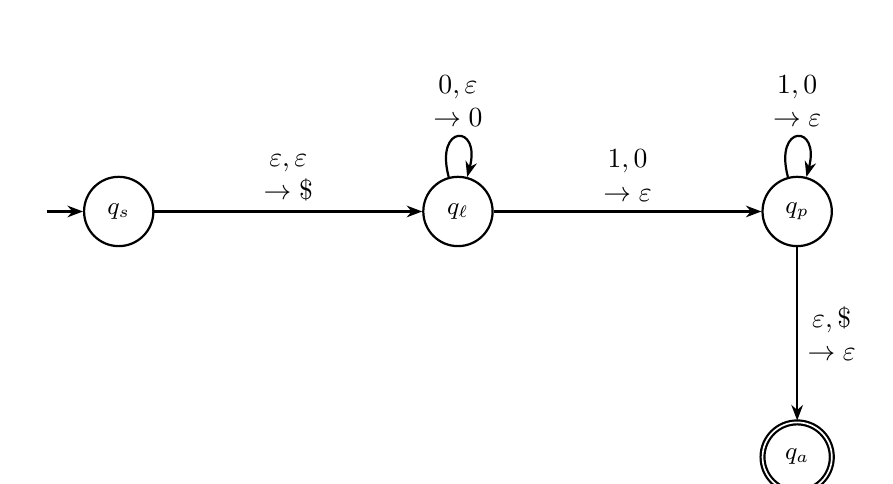
\begin{tikzpicture}[automaton,node distance=34mm]
  \node[state,initial] (qs) {$q_s$};
  \node[state,right=of qs] (ql) {$q_\ell$};
  \node[state,right=of ql] (qp) {$q_p$};
  \node[state,accepting,below=22mm of qp] (qa) {$q_a$};
  \path[->]
    (qs) edge node[align=center,above]{$\eps,\eps$\\$\to\mathdollar$} (ql)
    (ql) edge[loop above] node[align=center]{$0,\eps$\\$\to 0$} ()
         edge node[align=center,above]{$1,0$\\$\to\eps$} (qp)
    (qp) edge[loop above] node[align=center]{$1,0$\\$\to\eps$} ()
         edge node[align=center,right]{$\eps,\mathdollar$\\$\to\eps$} (qa);
\end{tikzpicture}
\end{center}
A label $a,x\to y$ means ``read $a$, pop $x$, push $y$''. On input $0011$,
after pushing $\mathdollar$ the stack is $00\mathdollar$ (top on the left);
each $1$ pops a $0$; a final $\eps$-move pops $\mathdollar$ and accepts.
\end{example}

\begin{example}[Balanced parentheses]
Let
\[
  L=\set{w\in\set{(,)}^*:w\text{ is balanced}}.
\]
Use states $q_s,q_\ell,q_a$, stack alphabet $\set{(,\mathdollar}$, and
\[
\begin{aligned}
  \transition(q_s,\eps,\eps)
    &=\set{(q_\ell,\mathdollar)},\\
  \transition(q_\ell,(,\eps)
    &=\set{(q_\ell,( )},\\
  \transition(q_\ell,),()
    &=\set{(q_\ell,\eps)},\\
  \transition(q_\ell,\eps,\mathdollar)
    &=\set{(q_a,\eps)}.
\end{aligned}
\]
Push on $($, pop on $)$, and accept by an $\eps$-move that pops the bottom
marker. Nondeterminism is not required. A copy dies if it tries to pop $($
when the top is $\mathdollar$, or if it reads $)$ with empty useful stack.
\end{example}

\subsection{PDAs and CFGs}
\begin{theorem}
A language is context-free if and only if some PDA recognizes it.
\end{theorem}

\begin{proof}[Proof idea]
($\Rightarrow$) From a CFG, a PDA keeps a sentential form on the stack, top
symbol being the next to expand. It nondeterministically replaces a variable
by a right-hand side, and matches terminals against the input.

($\Leftarrow$) From a PDA, a CFG has variables $A_{pq}$ meaning ``stack height
returns, going from state $p$ to state $q$''. Rules simulate a single PDA
move that pushes a symbol and later pops it, with an intermediate computation
in between.

Thus $\cfl=\set{\lang{P}:P\text{ is a PDA}}$.
\end{proof}

Acceptance by empty stack versus final state is equivalent for nondeterministic
PDAs: one extra state or marker converts either convention into the other.


\end{document}
